\documentclass{amsart}
\usepackage{graphicx}
\graphicspath{{./}}
\usepackage{hyperref}
\usepackage{csvsimple}
\usepackage{longtable}
\usepackage{epigraph}
\title{CONGRATULATIONS POPE FOR INTELLIGENCE ON DEMON BILL GATES' EVIL PLANS TO DESTROY HUMAN RACE}
\author{Zulfikar Moinuddin Ahmed}
\date{\today}
\begin{document}
\maketitle

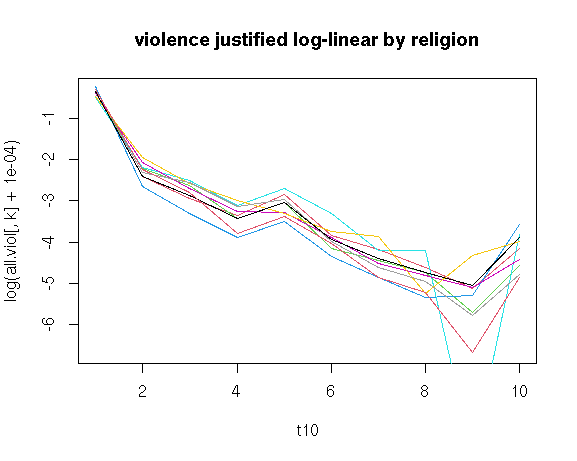
\includegraphics[scale=1.0]{violrel.png}

\section{All religions share identical moral views regarding violence}

One of my greatest scientific discoveries has been universality of moral values across the world.  The uniformity across religions for moral opinion here is quite close.  Statistically they are indistinguishable by my criteria for discrete variation by my Zulf chisquared independence test.  There is fine structure beyond exponential that we can see in the graphs.

\section{Application: Refute anti-Muslim propaganda}

I love my work having immediate applications, and the first is the observation that Muslim views of violence are virtually identical to Christian views of violence.

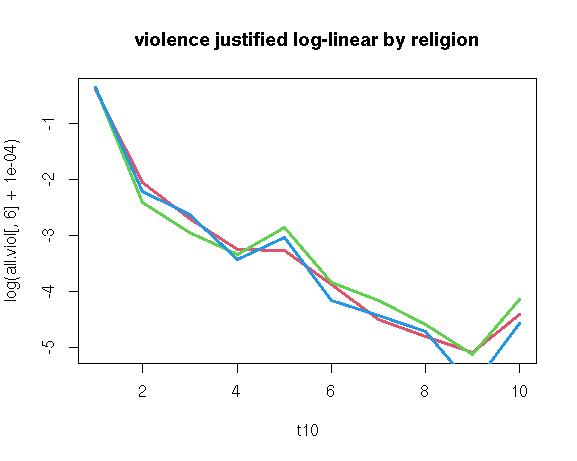
\includegraphics[scale=1.0]{musviol.jpg}

The red is Muslims; green is Catholics; blue Protestants.  Data are from WVS 7.

\end{document}
